
\chapter{Introduction and Background} 
\thispagestyle{myheadings} 
In this chapter, we first discuss some regular types of sensing systems 
used for guarding, tracking or surveilence, 
with a focus on the line-based and range-based sensors studied in this dissertation. 
% and we then introduce the two types of simplified sensing model studied in this thesis, 
Then, we conduct a literature study of the related work on sensor placement and 
coverage related problems. 
Lastly, some background knowledge of the theories and tools used in this paper will be given. 
\section{Some Examples of Sensing Systems} 
Sensor systems are ubiquitous. To list a few, systems of radar antennas 
or other sensor sources are frequently used as base stations for signal transmission, 
or intruder detection system (IDS) for monitoring hazards. 
Early intruder defense system can date back to ancient times, where 
watchtowers of the Great Wall of China are used as signal points. 
It can be seen as sensors from the broad sense 
since ancient soldiers lit woods to create smoke to inform others when invaders appear. 
% Surveilence or tracking cameras surveillance and tracking system, 
\begin{figure}[ht]
    \centering 
    \begin{subfigure}[b]{0.281\textwidth} 
        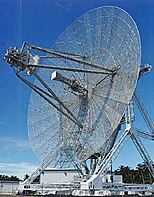
\includegraphics[width=\textwidth]{figures/Radar_antenna.jpg} 
        \caption{Radar antenna} 
        \label{fig:intro-radar} 
    \end{subfigure} 
    \begin{subfigure}[b]{0.48\textwidth} 
        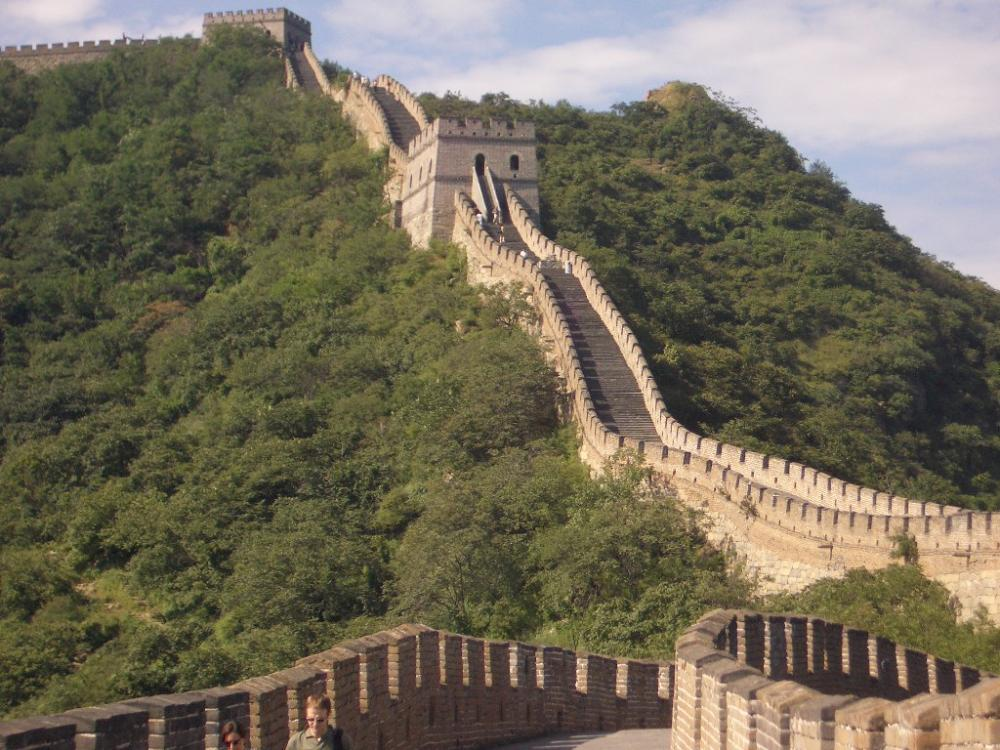
\includegraphics[width=\textwidth]{figures/great_wall.jpg} 
        \caption{Watch towers on the great wall} 
        \label{fig:intro-great_wall} 
    \end{subfigure}
    \caption{Two examples of intrusion detection system}
    \label{fig:intro-IDS}
\end{figure} 

On top of autonomous vehicles, sensor systems are indispensible for obstacle avoidance and interactions between vehicles, 
e.g., Tesla car (~\ref{fig:intro-tesla}) used 12 ultrasonic sensors 
near the front and rear bumper 
and later changed into a vision system with only cameras 
\footnote{\url{https://www.tesla.com/en_eu/support/transitioning-tesla-vision}}. 
TuSimple, an autonomous truck company, employs a combination of cameras, radars and lidars 
for their perception system \footnote{\\\url{https://www.tusimple.com/blogs/tusimple-1000-meter-perception-system}}. 

\begin{figure}[ht] 
    \centering 

    \begin{subfigure}[b]{0.49\textwidth} 
        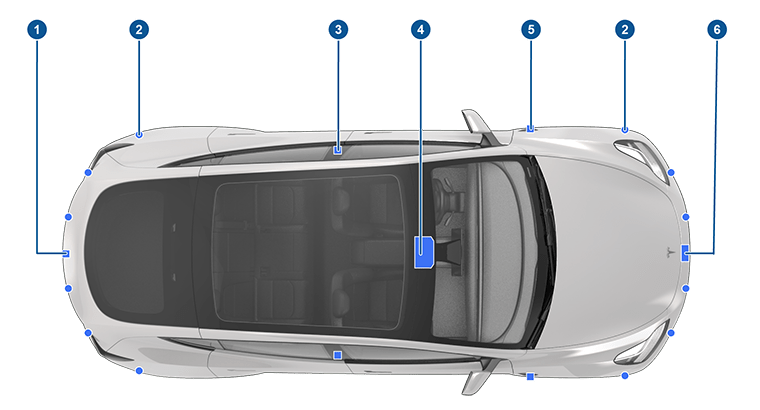
\includegraphics[width=\textwidth]{figures/tesla.png} 
        \caption{
        Tesla model Y's sensing system
        equipped with cameras (\circled{\small{1}}, 
        \circled{\small{3}}, 
        \circled{\small{4}}, \circled{\small{5}}),
        ultrasonic sensors \circled{\small{2}}, and a radar \circled{6}.
        }
        \label{fig:intro-tesla} 
    \end{subfigure} \hfill
    \begin{subfigure}[b]{0.4\textwidth} 
        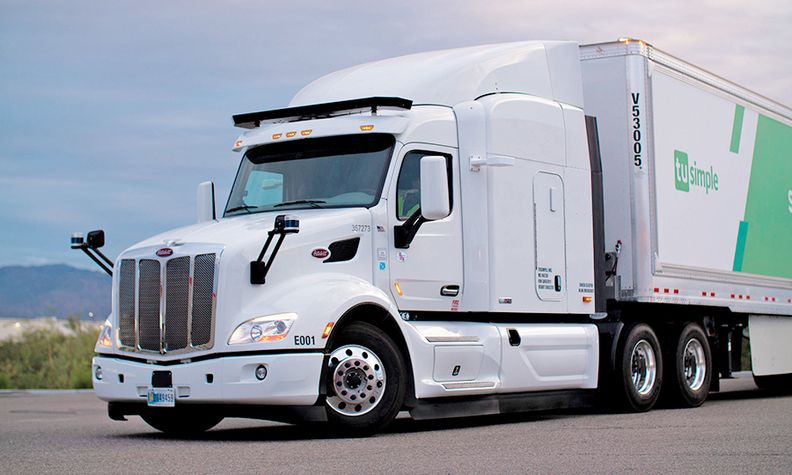
\includegraphics[width=\textwidth]{figures/tusimple.jpg} 
        \caption{TuSimple autonomous truck equipped with CMOS long-range cameras, 
        LiDARs and radars} 
        \label{fig:intro-truckcam} 
    \end{subfigure} 
    \caption{Sensor systems on autonomous vehicles}
    \label{fig:intro-autonomous-vehicles}
\end{figure} 

For surveilence or tracking systems, 
sensors like laser beams or cameras are deployed for applications like detecting thiefs, 
capturing motions, tracking poses and so on. 
\begin{figure}[ht] 
    \centering 
    
    % \begin{subfigure}[b]{0.55\textwidth} 
    %     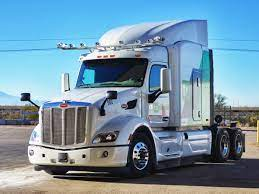
\includegraphics[width=\textwidth]{figures/truck_cam.jpeg} 
    %     \caption{Autonomous truck camera system} 
    %     \label{fig:intro_truckcam} 
    % \end{subfigure} 
    \begin{subfigure}[b]{0.41\textwidth} 
        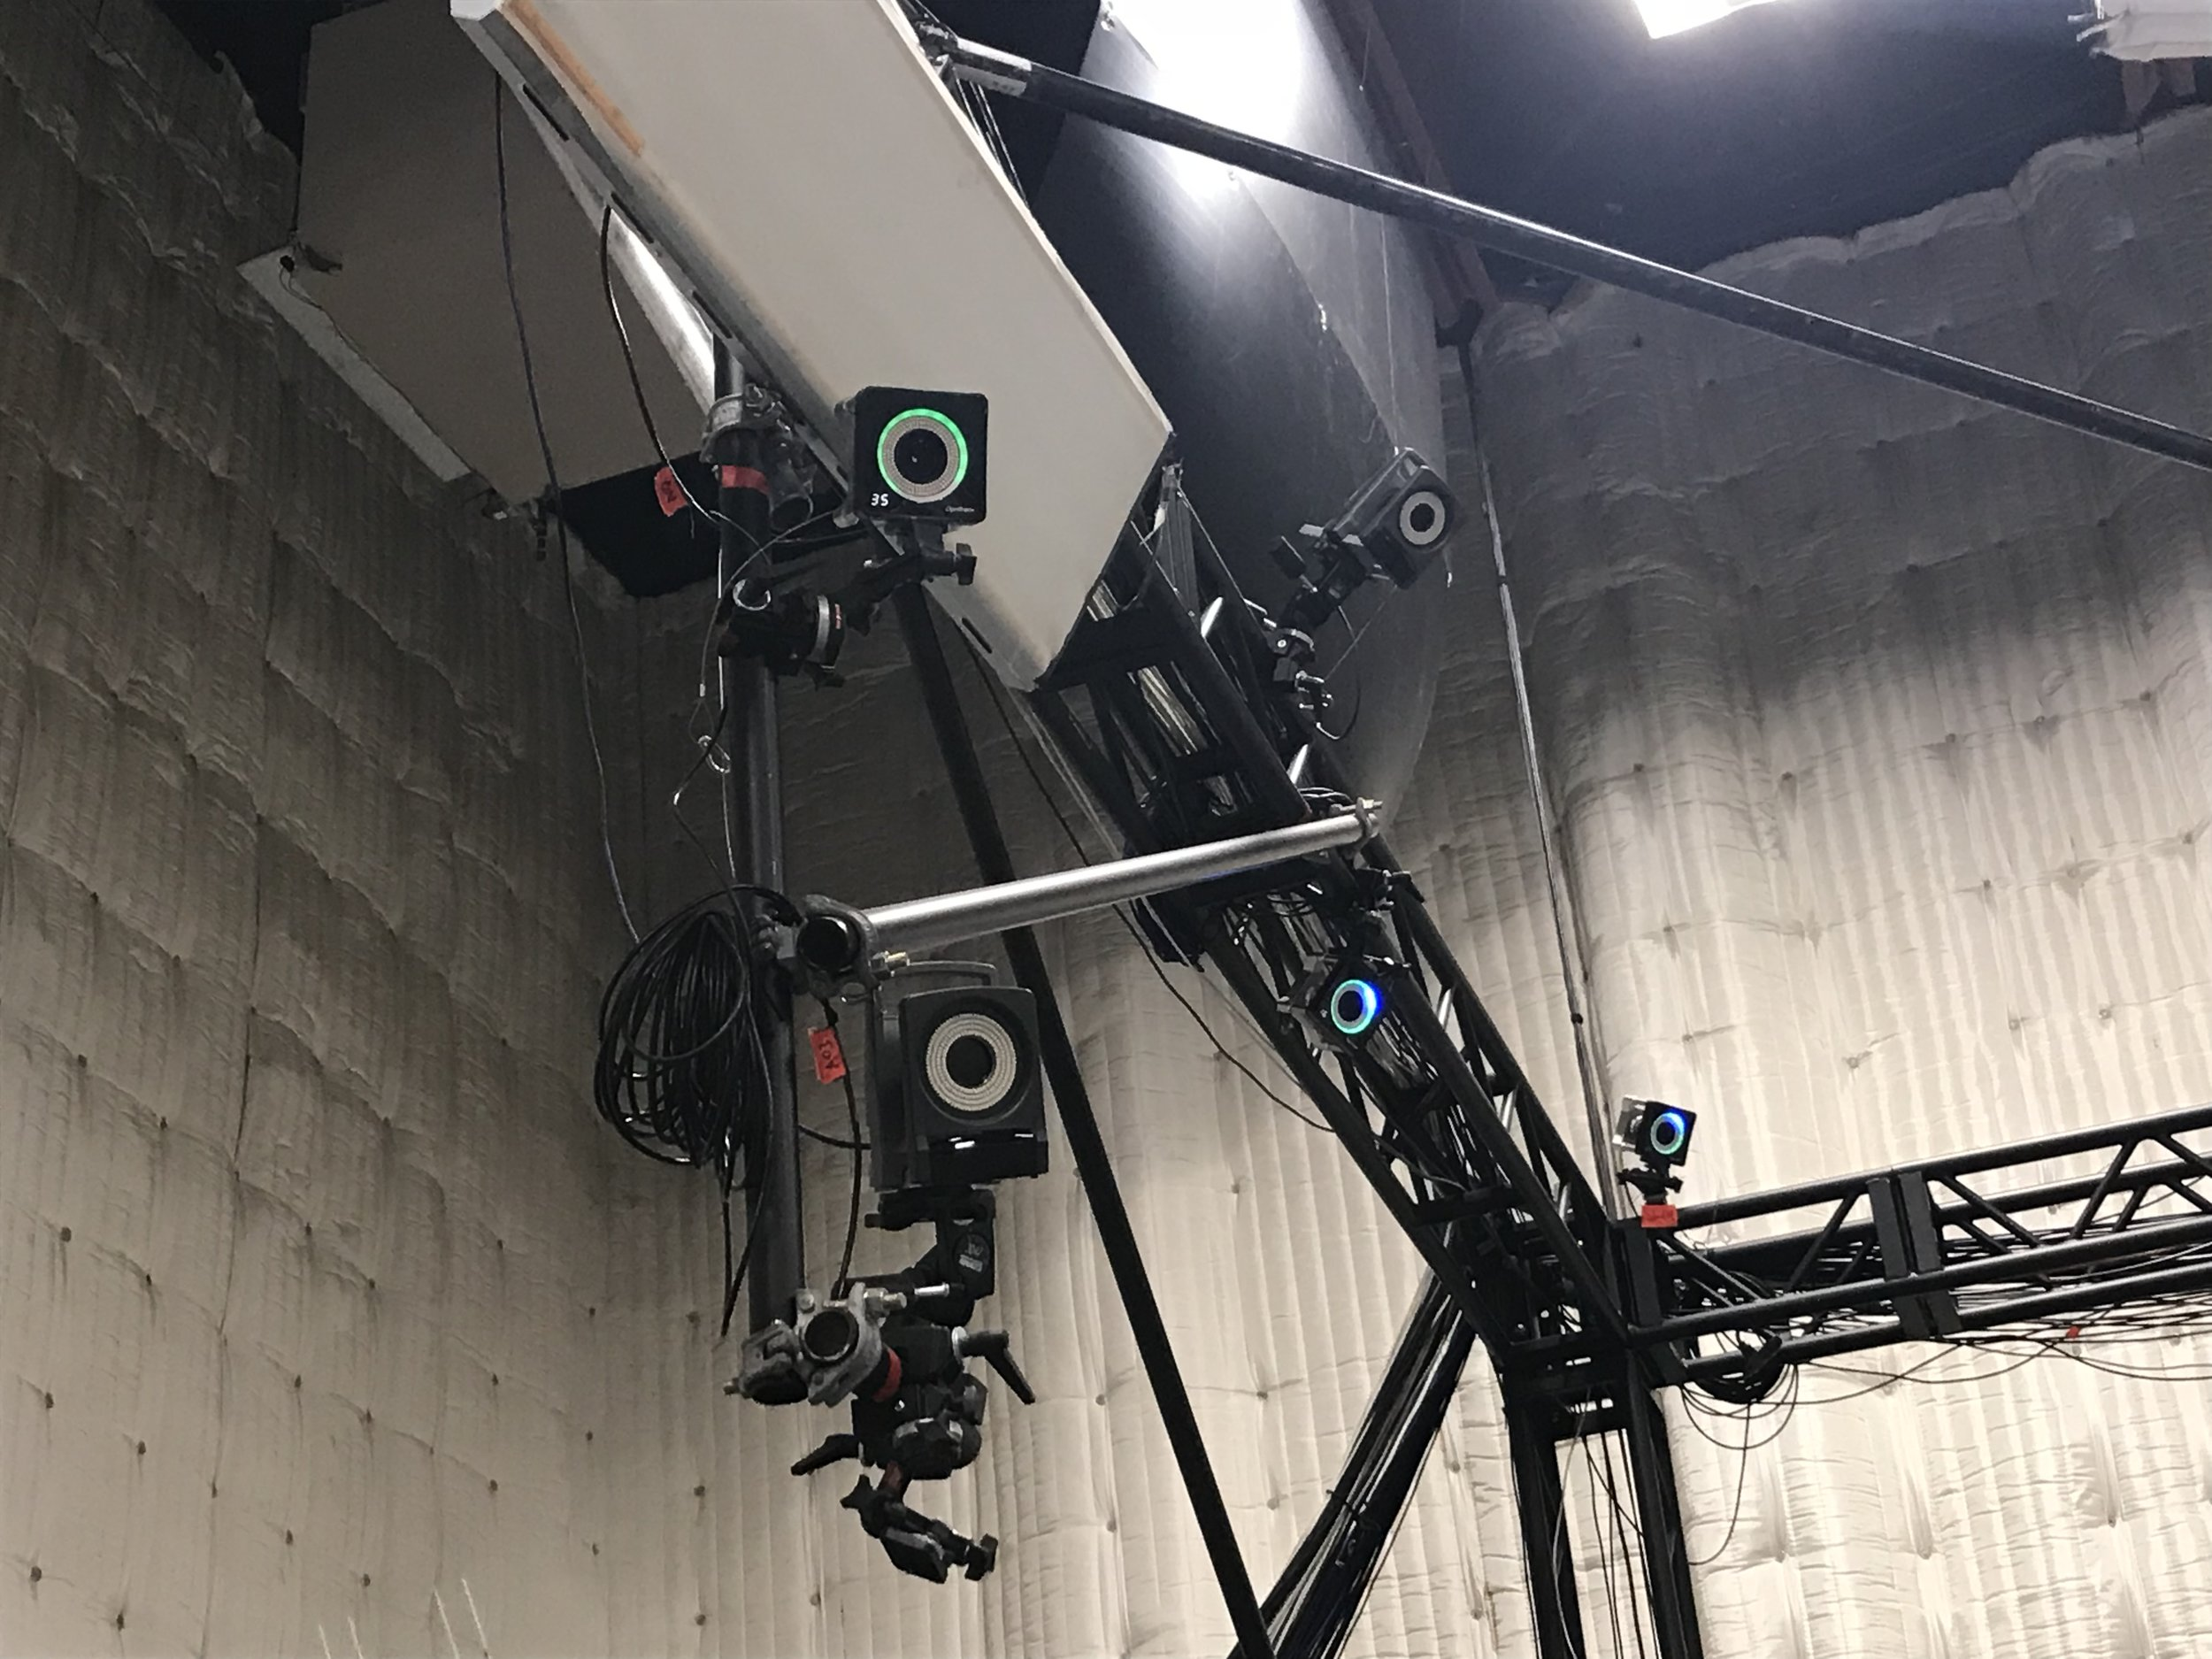
\includegraphics[width=\textwidth]{figures/optitrack.jpg} 
        \caption{Optical tracking system} 
        \label{fig:intro-optitrack} 
    \end{subfigure} 
    \hfill
    \begin{subfigure} [b]{0.46\textwidth} 
        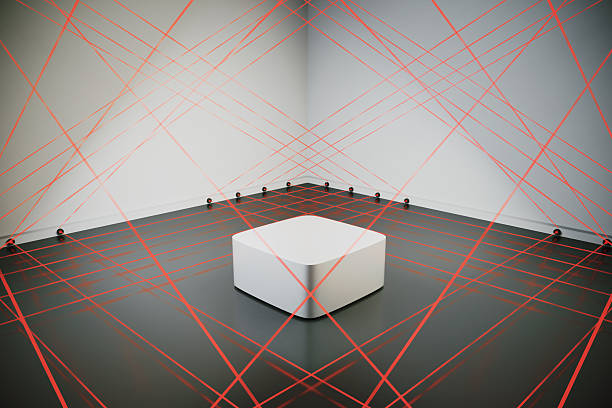
\includegraphics[width=\textwidth]{figures/laser.jpg} 
        \caption{Laser system} 
        \label{fig:intro-laser} 
    \end{subfigure} 
\end{figure}

\section{Background}
In this section, we discuss some background knowledge and terms used in this thesis,
they will be used without explaination in the later chapters. 

\subsection{NP-completeness and NP-hardness}
% In the area of optimization, which this thesis is focusing on, NP-hardness has the 
The definition of NP-completeness is taken from \cite{vazirani2001approximation}
\begin{definition}[NP-completeness]
    A language $L\in NP$ if there is a polynomial $p$ and a polynomial time bounded Turing machine M, 
    called the {\textit verifier}, such that for each string $x\in \{0, 1\}^*$: 
\begin{itemize}
    \item if $x\in L$, then there is a string $y$ (the certificate) of polynomially bounded length, i.e., $|y| \leq p(|x|)$,
    such that $M(x, y)$ accepts, and 
    \item if $x\notin L$, then for any string $y$, such that $|y|\leq p(|x|)$, $M(x,y)$ rejects.
\end{itemize}
\end{definition}

In the area of combinatorial optimization, and ${\bold{NP}}-optimization$ 
\subsection{Integer programming}

\section{Literature review} 
\subsection{Mobile sensing robot coverage control}
\subsection{Multi-robot coordination}
\subsection{Coverage-related problems in computational geometry}
\subsection{Sensor network}
